\documentclass[]{article}
\usepackage[brazilian]{babel}
\usepackage[utf8]{inputenc}
\usepackage[T1]{fontenc}
\usepackage{fancyhdr}
\usepackage{extramarks}
\usepackage{amsmath}
\usepackage{amsthm}
\usepackage{amsfonts}
\usepackage{tikz}
\usepackage[plain]{algorithm}
\usepackage{algpseudocode}
\usepackage{listings}
\usepackage{xcolor}
\usepackage{listings}
\usepackage{amssymb}

\definecolor{mGreen}{rgb}{0,0.6,0}
\definecolor{mGray}{rgb}{0.5,0.5,0.5}
\definecolor{mPurple}{rgb}{0.58,0,0.82}
\definecolor{backgroundColour}{rgb}{0.95,0.95,0.92}

\lstdefinestyle{CStyle}{
    belowcaptionskip=1\baselineskip,
    breaklines=true,
    frame=L,
    xleftmargin=\parindent,
    language=C,
    showstringspaces=false,
    basicstyle=\footnotesize\ttfamily,
    keywordstyle=\bfseries\color{green!40!black},
    commentstyle=\itshape\color{purple!40!black},
    identifierstyle=\color{blue},
    stringstyle=\color{orange},
}

\usetikzlibrary{automata,positioning}

%
% Basic Document Settings
%

\topmargin=-0.45in
\evensidemargin=0in
\oddsidemargin=0in
\textwidth=6.5in
\textheight=9.0in
\headsep=0.25in

\linespread{1.1}

\pagestyle{fancy}
\lhead{AVC, JPP, PC}
\chead{\hmwkClass\ (\hmwkClassInstructor\ \hmwkClassTime): \hmwkTitle}
\rhead{\firstxmark}
\lfoot{\lastxmark}
\cfoot{\thepage}

\renewcommand\headrulewidth{0.4pt}
\renewcommand\footrulewidth{0.4pt}

\setlength\parindent{0pt}

%
% Create Questão Sections
%

\newcommand{\enterProblemHeader}[1]{
    \nobreak\extramarks{}{Questão \arabic{#1} continua na próxima página\ldots}\nobreak{}
    \nobreak\extramarks{Questão \arabic{#1} (cont.)}{Questão \arabic{#1} continua na próxima página\ldots}\nobreak{}
}

\newcommand{\exitProblemHeader}[1]{
    \nobreak\extramarks{Questão \arabic{#1} (cont.)}{Questão \arabic{#1} continua na próxima página\ldots}\nobreak{}
    \stepcounter{#1}
    \nobreak\extramarks{Questão \arabic{#1}}{}\nobreak{}
}

\setcounter{secnumdepth}{0}
\newcounter{partCounter}
\newcounter{homeworkProblemCounter}
\setcounter{homeworkProblemCounter}{1}
\nobreak\extramarks{Questão \arabic{homeworkProblemCounter}}{}\nobreak{}

%
% Homework Questão Environment
%
% This environment takes an optional argument. When given, it will adjust the
% problem counter. This is useful for when the problems given for your
% assignment aren't sequential. See the last 3 problems of this template for an
% example.
%
\newenvironment{homeworkProblem}[1][-1]{
    \ifnum#1>0
        \setcounter{homeworkProblemCounter}{#1}
    \fi
    \section{Questão \arabic{homeworkProblemCounter}}
    \setcounter{partCounter}{1}
    \enterProblemHeader{homeworkProblemCounter}
}{
    \exitProblemHeader{homeworkProblemCounter}
}

%
% Homework Details
%   - Title
%   - Due date
%   - Class
%   - Section/Time
%   - Instructor
%   - Author
%

\newcommand{\hmwkTitle}{Lista 1}
\newcommand{\hmwkDueDate}{16 de outubro de 2019}
\newcommand{\hmwkClass}{Programação Modular}
\newcommand{\hmwkClassTime}{}
\newcommand{\hmwkClassInstructor}{Professor Flavio Bevilacqua}

% \setlength{\textfloatsep}{1in}
\newcommand{\hmwkAuthorName}{

\begin{tabular}{c}\textbf{Antônio Vasconcellos Chaves} \\ Engenharia da Computaçāo \\ Pontifícia Universidade Católica \\ do Rio de Janeiro \\ Rio de Janeiro, RJ 22451-900 \\ antoniovasconcelloschaves@gmail.com \end{tabular}\and

\begin{tabular}{c}\textbf{João Pedro Paiva} \\ Ciência da Computaçāo \\ Pontifícia Universidade Católica \\ do Rio de Janeiro \\ Rio de Janeiro, RJ 22451-900 \\ joaopedrordepaiva@gmail.com \end{tabular}\and

\\[\baselineskip]\begin{tabular}{c}\textbf{Pedro Moreira Costa} \\ Engenharia da Computaçāo \\ Pontifícia Universidade Católica \\ do Rio de Janeiro \\ Rio de Janeiro, RJ 22451-900 \\ pedromoreiramcosta@gmail.com \end{tabular}

}

%
% Title Page
%

\title{
    \vspace{2in}
    \textmd{\textbf{\hmwkClass:\ \hmwkTitle}}\\
    \normalsize\vspace{0.1in}\small{Entrega\ no dia\ \hmwkDueDate\ às 17h}\\
    \vspace{0.1in}\large{\textit{\hmwkClassInstructor\ \hmwkClassTime}}
    \vspace{1.25in}
}

\author{\hmwkAuthorName}
\date{}

\renewcommand{\part}[1]{\textbf{\large Parte \Alph{partCounter}}\stepcounter{partCounter}\\}

%
% Various Helper Commands
%

% Useful for algorithms
\newcommand{\alg}[1]{\textsc{\bfseries \footnotesize #1}}

% For derivatives
\newcommand{\deriv}[1]{\frac{\mathrm{d}}{\mathrm{d}x} (#1)}

% For partial derivatives
\newcommand{\pderiv}[2]{\frac{\partial}{\partial #1} (#2)}

% Integral dx
\newcommand{\dx}{\mathrm{d}x}

% Alias for the Solution section header
\newcommand{\solution}{\textbf{\large Solução}}

% Probability commands: Expectation, Variance, Covariance, Bias
\newcommand{\E}{\mathrm{E}}
\newcommand{\Var}{\mathrm{Var}}
\newcommand{\Cov}{\mathrm{Cov}}
\newcommand{\Bias}{\mathrm{Bias}}

\begin{document}

\maketitle

\pagebreak

\begin{homeworkProblem}

    Explique com um exemplo o conceito de callback.

    \vspace{\baselineskip}
    \textbf{Solução}

    Callback é o termo usado para quando ao ter os dados requisitados, enviados pelo cliente, ainda há requisitos não preenchidos que não são obrigatórios. Por exemplo, em um cadastro, o servidor precisa das informações (nome, sobrenome e CPF) do cliente. O cliente esquece de preencher o CPF. Então o servidor volta/gera para interface com um aviso de que aquele campo é de preenchimento obrigatório.

\end{homeworkProblem}

\vspace{\baselineskip}

\begin{homeworkProblem}

    Apresente um requisito funcional bem formulado, derivado de um requisito não funcional, diferente do exemplo de login visto em aula.

    \vspace{\baselineskip}
    \textbf{Solução}

    A necessidade que a solução seja descentralizada, por exemplo. Pois torna necessária a implementação de módulos para estabelecer a conexão entre os nós do sistema distribuído.

\end{homeworkProblem}

\vspace{\baselineskip}

\begin{homeworkProblem}

    Um bom acoplamento resulta em um bom encapsulamento. Certo, errado, tipo assim, justifique.

    \vspace{\baselineskip}
    \textbf{Solução}

    Errado. Ambos estão relacionados mas não têm influência um sobre o outro. O acoplamento pode ser feito com diversos parâmetros por função e conectores complexos e, mesmo assim, manter a integridade da estrutura a ser protegida e ter fácil manutenção se tudo que está relacionado à parte protegida encontra-se no mesmo local.

\end{homeworkProblem}

\vspace{\baselineskip}

\begin{homeworkProblem}

    Nem toda coesão funcional é lógica. Certo, errado, tipo assim (depende), justifique.

    \vspace{\baselineskip}
    \textbf{Solução}

    Errado. Como a coesão funcional implica que os elementos interdependem em torno de uma funcionalidade podemos afirmar que também interdependem em torno do conceito lógico associado a ela.

\end{homeworkProblem}

\vspace{\baselineskip}

\begin{homeworkProblem}

    É possível existir mais de um módulo de definição para um módulo de implementação? Porque alguém faria isso?

    \vspace{\baselineskip}
    \textbf{Solução}

    Sim. Para alterar a visibilidade dos métodos e atributos, ou seja, das funções e variáveis presentes naquele módulo.

\end{homeworkProblem}

\vspace{\baselineskip}

\begin{homeworkProblem}

    Faça modelo, exemplo e assertivas de uma matriz dinâmica tridimensional que armazena árvores binárias que referenciam listas de matrizes genéricas bidimensionais.

    \vspace{\baselineskip}
    \textbf{Solução}

    \begin{figure}[h]
        \centering
        \caption{Modelo físico da matriz dinâmica tridimensional que armazena árvores binárias que referenciam listas de matrizes genéricas bidimensionais.}
        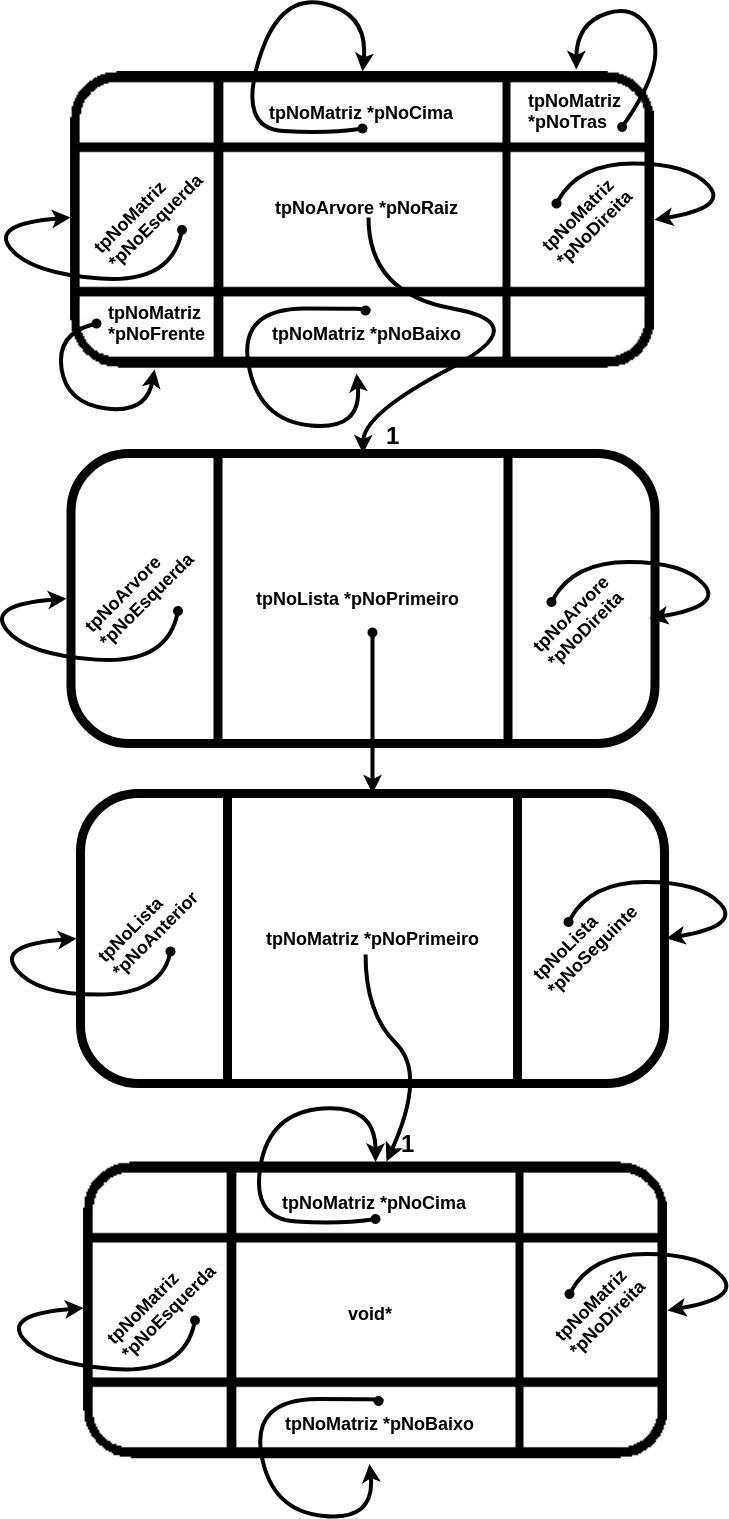
\includegraphics[width=0.479\textwidth]{modelo.png}
    \end{figure}

    \begin{figure}[h]
        \centering
        \caption{Exemplo físico da matriz dinâmica tridimensional que armazena árvores binárias que referenciam listas de matrizes genéricas bidimensionais.}
        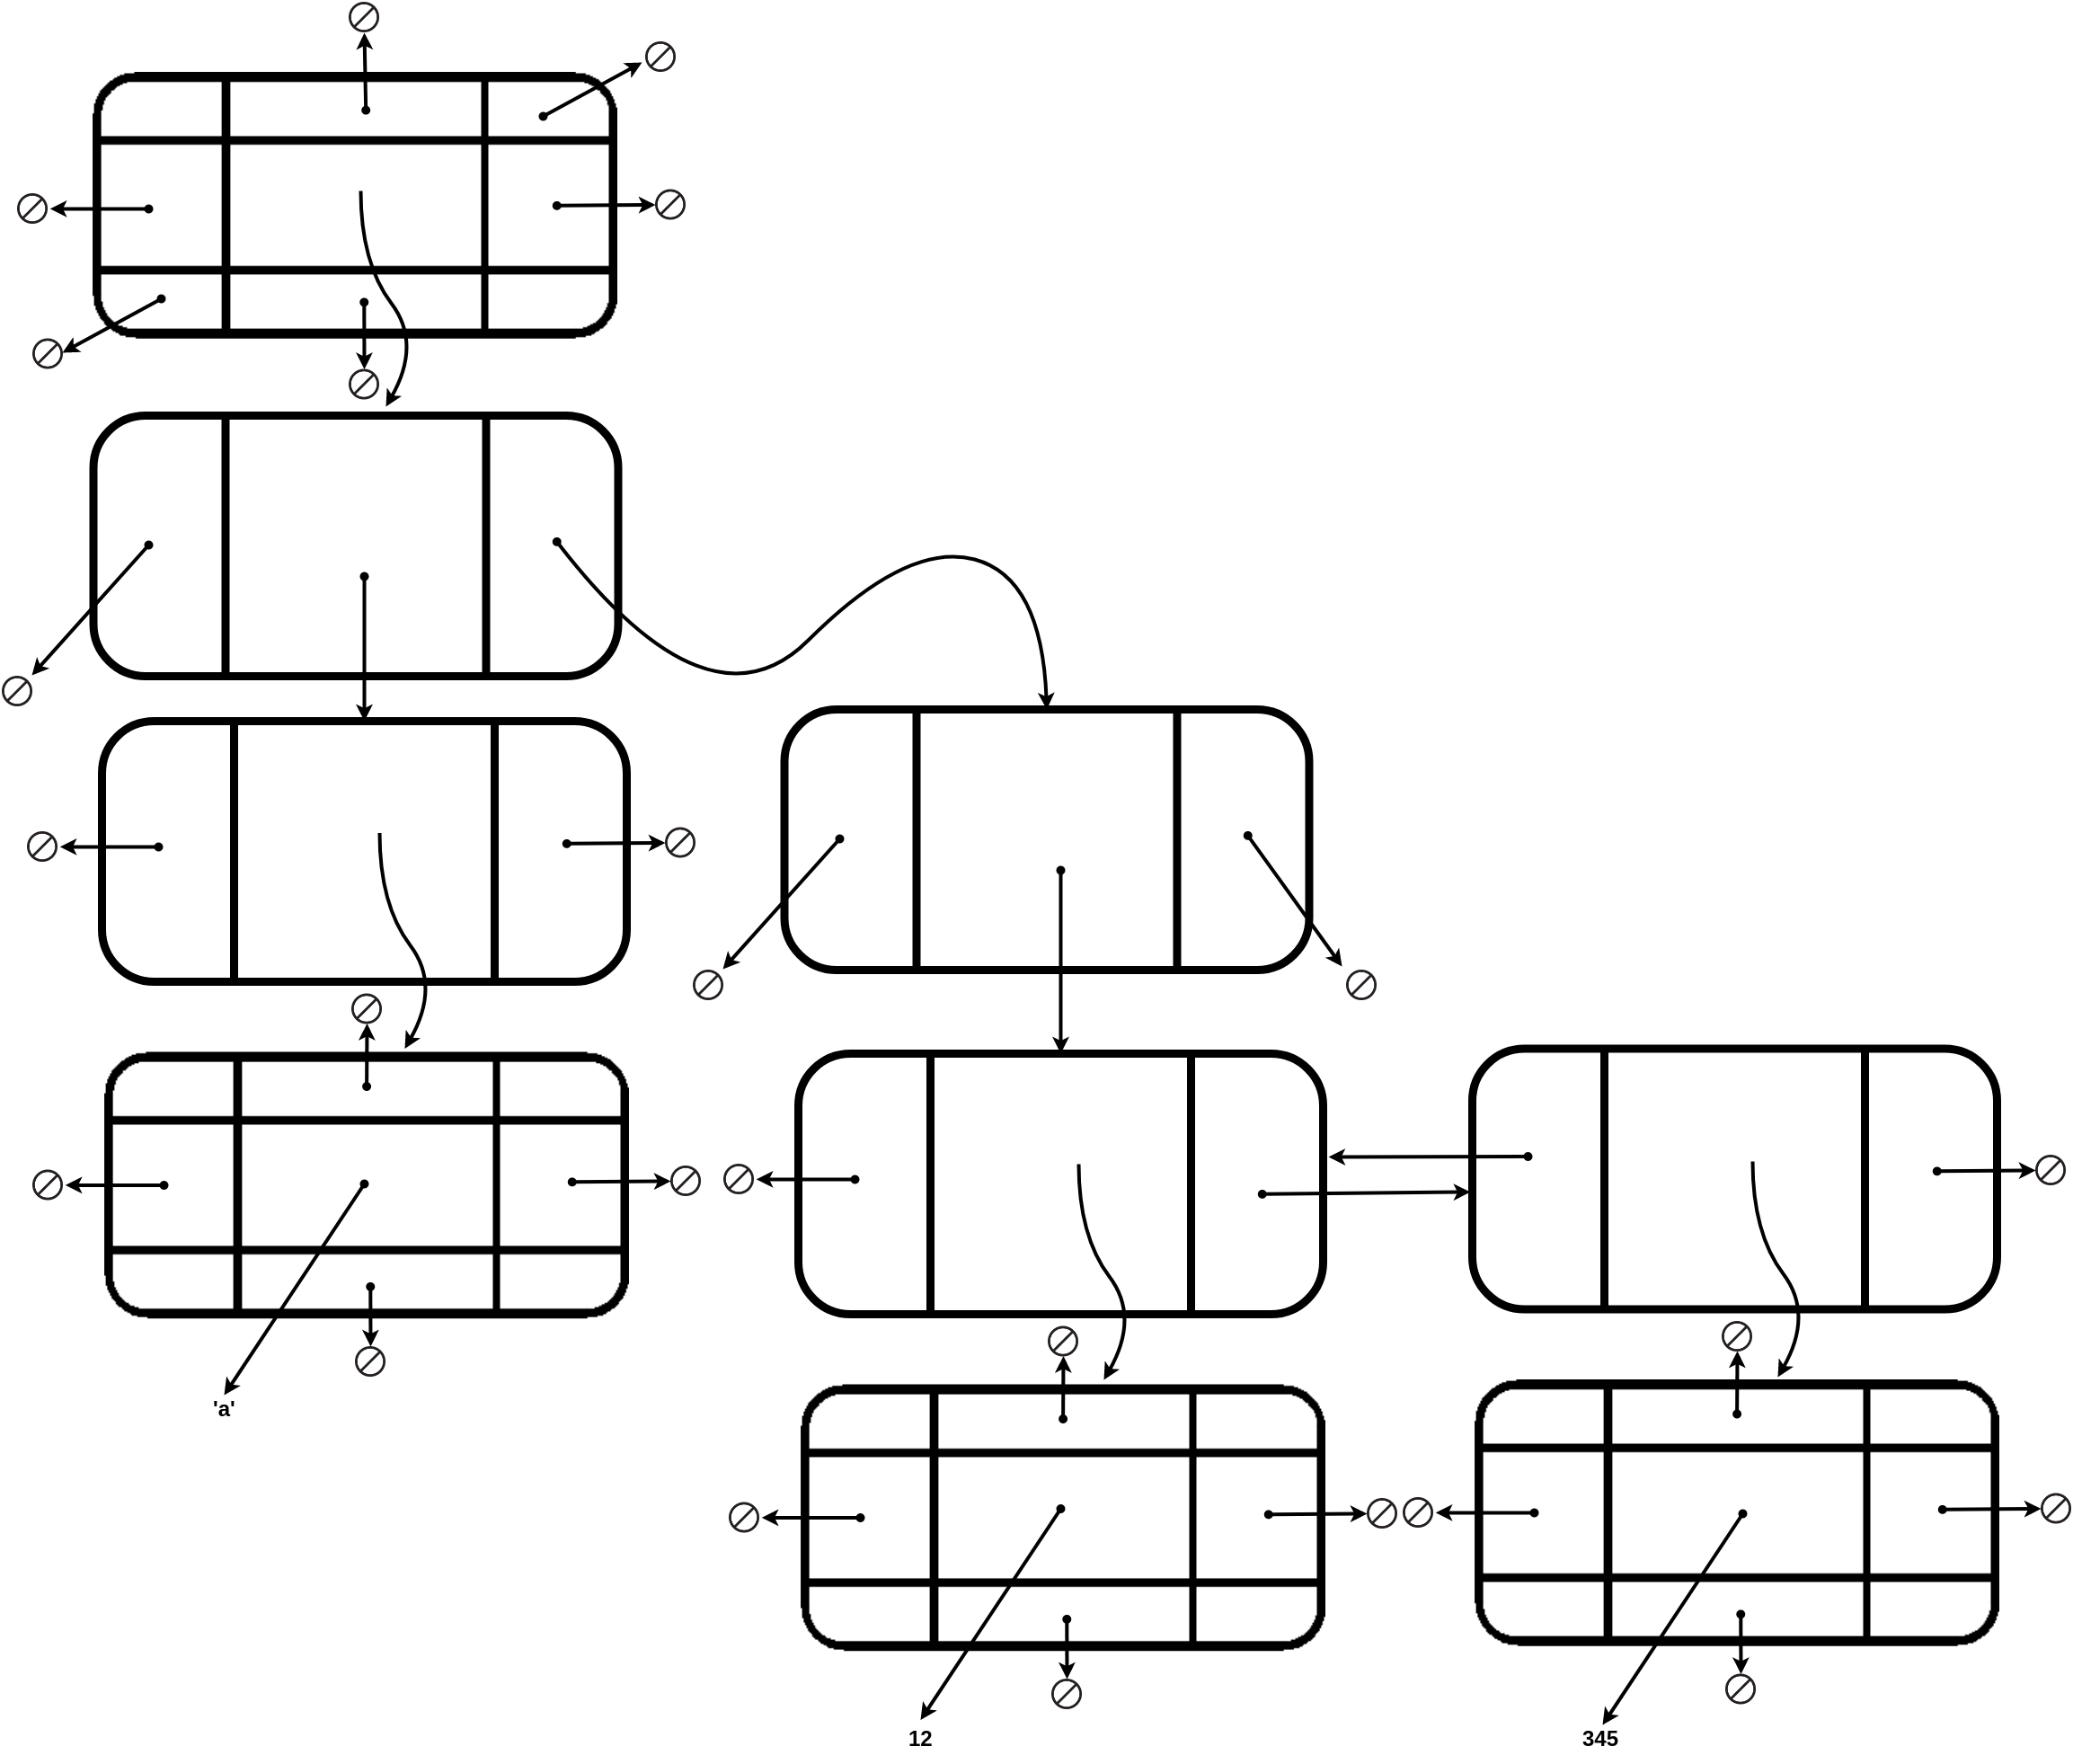
\includegraphics[width=\textwidth]{exemplo.png}
    \end{figure}

    \begin{itemize}

        \item \sloppy$\forall \textrm{ nó } pNo \in \textrm{matriz dinâmica tridimensional : } pNo \rightarrow pNoDireita \ != \ NULL \implies pNo \rightarrow pNoDireita \rightarrow pNoEsquerda == pNo$
        \item \sloppy$\forall \textrm{ nó } pNo \in \textrm{matriz dinâmica tridimensional : } pNo \rightarrow pNoEsquerda \ != \ NULL \implies pNo \rightarrow pNoEsquerda \rightarrow pNoDireita == pNo$
        \item \sloppy$\forall \textrm{ nó } pNo \in \textrm{matriz dinâmica tridimensional : } pNo \rightarrow pNoCima \ != \ NULL \implies pNo \rightarrow pNoCima \rightarrow pNoBaixo == pNo$
        \item \sloppy$\forall \textrm{ nó } pNo \in \textrm{matriz dinâmica tridimensional : } pNo \rightarrow pNoBaixo \ != \ NULL \implies pNo \rightarrow pNoBaixo \rightarrow pNoCima == pNo$
        \item \sloppy$\forall \textrm{ nó } pNo \in \textrm{matriz dinâmica tridimensional : } pNo \rightarrow pNoFrente \ != \ NULL \implies pNo \rightarrow pNoFrente \rightarrow pNoTras == pNo$
        \item \sloppy$\forall \textrm{ nó } pNo \in \textrm{matriz dinâmica tridimensional : } pNo \rightarrow pNoTras \ != \ NULL \implies pNo \rightarrow pNoTras \rightarrow pNoFrente == pNo$
        \item $\forall \textrm{ nó } pNo \in $ árvore binária : a referência para filho à esquerda de um nó tem como destino a raiz da sub-árvore à esquerda
        \item $\forall \textrm{ nó } pNo \in $ árvore binária : a referência para filho à direita de um nó tem como destino a raiz da sub-árvore à direita
        \item $\forall \textrm{ nó } pNo \in $ árvore binária : o conjunto de nós alcançáveis a partir da raiz da sub-árvore à esquerda é disjunto do conjunto de nós alcançáveis a partir da raiz da sub-árvore à direita
        \item $\forall \textrm{ nó } pNo \in $ árvore binária : não existe caminho na árvore que leve de $pNo \rightarrow pNoEsquerda$ ou $pNo \rightarrow pNoDireita$ a $pNo$
        \item \sloppy$\forall \textrm{ nó } pNo \in \textrm{lista : } pNo \rightarrow pNoDireita \ != \ NULL \implies pNo \rightarrow pNoDireita \rightarrow pNoEsquerda == pNo$
        \item \sloppy$\forall \textrm{ nó } pNo \in \textrm{lista : } pNo \rightarrow pNoEsquerda \ != \ NULL \implies pNo \rightarrow pNoEsquerda \rightarrow pNoDireita == pNo$
        \item \sloppy$\forall \textrm{ nó } pNo \in \textrm{matriz genérica bidimensional : } pNo \rightarrow pNoDireita \ != \ NULL \implies pNo \rightarrow pNoDireita \rightarrow pNoEsquerda == pNo$
        \item \sloppy$\forall \textrm{ nó } pNo \in \textrm{matriz genérica bidimensional : } pNo \rightarrow pNoEsquerda \ != \ NULL \implies pNo \rightarrow pNoEsquerda \rightarrow pNoDireita == pNo$
        \item \sloppy$\forall \textrm{ nó } pNo \in \textrm{matriz genérica bidimensional : } pNo \rightarrow pNoCima \ != \ NULL \implies pNo \rightarrow pNoCima \rightarrow pNoBaixo == pNo$
        \item \sloppy$\forall \textrm{ nó } pNo \in \textrm{matriz genérica bidimensional : } pNo \rightarrow pNoBaixo \ != \ NULL \implies pNo \rightarrow pNoBaixo \rightarrow pNoCima == pNo$        

    \end{itemize}

\end{homeworkProblem}

\vspace{\baselineskip}

\begin{homeworkProblem}

    Explique como é possível alterar o idimoa utilizado nas telas de uma aplicação sem esse ter sido previsto ao longo do desenvolvimento e sem haver a necessidade de compilar e linkeditar novamente a aplicação.

    \vspace{\baselineskip}
    \textbf{Solução}

    Podemos acoplar todo texto que será exibido no programa em uma biblioteca dinâmica (DLL), que é ligada em tempo de execução. Assim, caso futuramente seja uma necessidade o uso de outro idioma, basta escrever uma nova biblioteca referente ao mesmo, sem que seja preciso recompilar a aplicação.


\end{homeworkProblem}

\vspace{\baselineskip}

\begin{homeworkProblem}

    Dê exemplo de uma hipótese e explique em que isto auxilia no desenvolvimento de uma aplicação.

    \vspace{\baselineskip}
    \textbf{Solução}

    A validação de CPFs será feita no front-end da aplicação. Por esta hipótese sabe-se que não será necessário validar CPFs no back-end pois o mesmo foi feito no front-end.


\end{homeworkProblem}

\vspace{\baselineskip}

\begin{homeworkProblem}

    É possível utilizar variáveis globais como itens de interface fornecidos por terceiros? Mostre como (caso sim).

    \vspace{\baselineskip}
    \textbf{Solução}


\end{homeworkProblem}

\vspace{\baselineskip}

\begin{homeworkProblem}

    Explique se existe diferença entre requisito inverso e restrição.

    \vspace{\baselineskip}
    \textbf{Solução}

    Existe sim diferença entre requisito inverso e restrição. Requisito inverso é aquilo que não será feito. Por exemplo, "Não implementaremos o login porque não foi pedido". Rrestrições são regras que restringem as alternativas de solução de um problema. Por exemplo, "A aplicação deve ser redigida em C++".

\end{homeworkProblem}

\vspace{\baselineskip}

\begin{homeworkProblem}

    Um programa deve ser capaz de ler um documento de texto e criar um índice remissivo para cada substantivo encontrado. No índice remissivo é apresentada a lista de páginas e que a palavra é encontrada. Elabore a arquitetura modularizada deste programa (tal como foi vista na disciplina) considerando a criação de um tipo abstrato de dados para a estrutura principal a ser acoplada na aplicação. Neste tipo abstrato de dados deve ser utilizada a estrutura Lista Duplamente Encadeada com Cabeça.

    \vspace{\baselineskip}
    \textbf{Solução}

    \begin{figure}[h]
        \centering
        \caption{Arquitetura modularizada do programa que lê um documento de texto e cria um índice remissivo para cada substantivo encontrado.}
        
\includegraphics[width=0.193\textwidth]{arquiteturalistacomcabeca.png}
    \end{figure}

\end{homeworkProblem}

\vspace{\baselineskip}

\begin{homeworkProblem}

    Uma estrutura de chamadas de funções pode ser simultaneamente recursiva direta, indireta e gerar dependência circular entre módulos. Comente essa afirmação.

    \vspace{\baselineskip}
    \textbf{Solução}

    Um arco de chamadas não pode ser simultaneamente recursivo direto e indireto, mas pode ser recursivo indireto com trechos de recursão direta. Dependência circular possui mais relação com os módulos dos quais funções são chamadas no arco de chamadas do que as próprias funções chamadas. Um arco recursivo indireto pode gerar dependência circular, quando pelo menos uma função de outro módulo é chamada entre chamadas de uma mesma função. Mas um arco recursivo direto não pode gerar dependência circular.


\end{homeworkProblem}

\vspace{\baselineskip}

\begin{homeworkProblem}

    Dê um exemplo de função morta existente nos seus trabalhos. Justifique sua resposta.

    \vspace{\baselineskip}
    \textbf{Solução}


\end{homeworkProblem}

\vspace{\baselineskip}

\begin{homeworkProblem}

    Dado o seguinte requisito funcional: "Após o término da entrada das notas dos alunos na funcionalidade 'Apresentar Situação Final', a Média Final é calculada e apresentada na tela.". Avalie a necessidade da criação de um requisito inverso. Caso seja necessário, apresente este requisito e explique sua necessidade. Caso não seja necessário, explique a razão de não especificar este requisito.

    \vspace{\baselineskip}
    \textbf{Solução}

    Requisitos inversos são incluídos, geralmente, para eliminar ambiguidades. No requisito apresentado, não está claro qual Média Final deve ser calculada. Pode ser a Média Final de cada aluno ou de todos os alunos juntos. Também não está claro como a média deve ser calculada. Um requisito que poderia ser adicionado para esclarecer é: "esta aplicação não calcula a média de todos os alunos juntos, a média de cada aluno será calculada por (G1 + G2 + 2*T1)/4".

\end{homeworkProblem}

\begin{homeworkProblem}

    Especifique as asssertivas de entrada e saída de uma função que é armazenada no cabeça de uma lista para ser utilizada na exclusão do conteúdo apontado por um nó.

    \vspace{\baselineskip}
    \textbf{Solução}


\end{homeworkProblem}

\begin{homeworkProblem}

    A validação de requisitos é feita pela equipe técnica junto com o cliente. Certo/Errado. Justifique.

    \vspace{\baselineskip}
    \textbf{Solução}

    Certo. Após elicitar do cliente aquilo que ele deseja, documentar a elicitação e verificar se aquilo que o cliente deseja é factível, o Analista de Requisitos valida os requisitos documentados com o cliente.


\end{homeworkProblem}

\begin{homeworkProblem}

    Explique o que um gerente de configuração de software faz em um processo de desenvolvimento.

    \vspace{\baselineskip}
    \textbf{Solução}

    O gerente de configuração de software maneja baselines e ambientes de configuração.


\end{homeworkProblem}

\begin{homeworkProblem}

    "O relatório deve ter no máximo dez linhas por página". Requisito funcional, não funcional, restrição ou hipótese? Justifique.

    \vspace{\baselineskip}
    \textbf{Solução}

    Requisito não funcional. Pois descreve algo que deve ser feito, mas não está relacionado a uma funcionalidade específica.

\end{homeworkProblem}

\begin{homeworkProblem}

    Mostre através de um exemplo como é possível com um único módulo de definição gerar interfaces personalizadas para cada módulo cliente.

    \vspace{\baselineskip}
    \textbf{Solução}

    O seguinte código de um módulo de definição:

    \lstinputlisting[style=CStyle]{M1.h}

    gera \lstinputlisting[style=CStyle]{resultado1.c} com este trecho presente no módulo cliente:

    \lstinputlisting[style=CStyle]{MS.c}

    e gera \lstinputlisting[style=CStyle]{resultado2.c} com o seguinte trecho presente em outro módulo cliente:

    \lstinputlisting[style=CStyle]{MC.c}


\end{homeworkProblem}

\begin{homeworkProblem}

    Um valor somente declarado pode estar também definido? Certo/errado. Justifique.

    \vspace{\baselineskip}
    \textbf{Solução}

    **NUM MESMO MÓDULO!!**

\end{homeworkProblem}

\begin{homeworkProblem}

    É possível declarar sem definir? Porque alguém faria isso?

    \vspace{\baselineskip}
    \textbf{Solução}

    Sim. Para fazer referência a uma variável definida externamente, em outro módulo, que será ligada em tempo de linkedição, caso se trate de uma biblioteca estática, ou de execução, tratando-se de uma biblioteca dinâmica.

\end{homeworkProblem}

\begin{homeworkProblem}

    O encapsulamento sempre protege os dados. Certo/errado. Justifique.

    \vspace{\baselineskip}
    \textbf{Solução}

    Errado. Por mais que o encapsulamento tenha sido perfeito, ainda pode-se acessar o espaço de memória de algum dado e mexer nele, já que C é uma linguagem de baixo nível.

\end{homeworkProblem}


\end{document}
